\newpage
\section{Pianificazione}
I membri del gruppo, con l'obbiettivo di agevolare lo sviluppo del progetto, hanno deciso congiuntamente di suddividere il carico di lavoro in 6 periodi:
\begin{itemize}
	\item \ARM;
	\item \ARD;
	\item \PA;
	\item \PD;
	\item \COD;
	\item \VV.
\end{itemize}

Ad ognuno dei membri saranno assegnate delle attività principali da svolgere in un determinato periodo. Ognuno avrà dunque associato un \termine{diagramma di Gantt} al fine di agevolargli la visione e la comprensione delle tempistiche e delle scadenze delle varie attività assegnategli.
Ogni attività potrà, a sua volta, essere suddivisa in sotto-attività ed avere, o meno, forte dipendenze con altre attività.\\
Saranno inoltre definite delle \termine{milestone} esterne ed interne che coincideranno, rispettivamente, con le date di scadenza per la consegna dei documenti e con le scadenze per le revisioni stabilite dai membri del gruppo.
Ogni periodo, tra quelli sopraelencati, terminerà sempre con una \termine{milestone}.\\

Le diverse attività saranno rappresentate nel \termine{diagramma di Gantt} in termini temporali mediante linee blu.

\subsection{Suddivisione delle attività}

\subsubsection{\ARM}
Periodo: dal 13/12/2016 all'11/01/2017. \\

L'inizio del periodo di \ARM\ corrisponde all'inizio del progetto. In questa fase il gruppo deve scegliere un \termine{capitolato} e cominciare a lavorare con il fine ultimo di aggiudicarselo.\\
Ciò comporta la stesura dei seguenti documenti:
 \begin{itemize}
 \item Esterni:
 	\begin{itemize}
 	 \item \AdR
 	 \item \PdP
	 \item \PdQ
 	\end{itemize}
 \item  Interni:
	\begin{itemize}
	\item \SdF
	\item \NdP
	\end{itemize} 
 \end{itemize}
 Il carico di lavoro viene suddiviso principalmente tra i ruoli di \An, \Am, \Ver\ e \Pm.
 Il periodo termina con una milestone esterna, corrispondente alla consegna dei documenti per la \RR.
 
 \begin{figure}[H]
	\centering 
	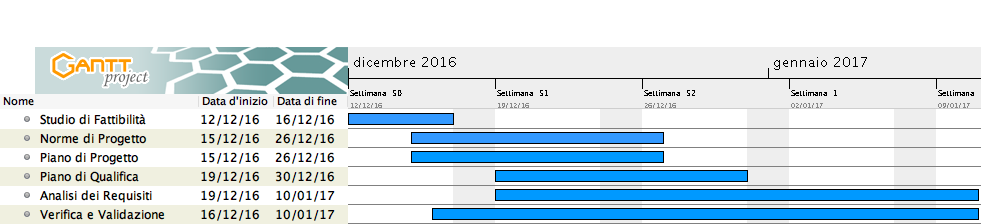
\includegraphics[scale=0.4]{Immagini/Gantt/ARM.png}
	\caption{Diagramma di Gantt, \ARM}
\end{figure}

\subsection{\ARD}
Periodo: dal 12/01/2017 al 03/02/2017 \\

Questo periodo inizia subito dopo la consegna dei documenti per la \RR. Il termine corrisponde ad una \termine{milestone} interna che coincide con l'inizio del periodo successivo, la \PA.\\
Il \termine{gruppo} in questo periodo si impegnerà a consolidare ed ampliare, in modo più dettagliato, i requisiti richiesti per lo svolgimento del progetto.\\
Verranno inoltre effettuate le modifiche necessarie, rilevate in seguito all'esito della \RR\, nei vari documenti.\\
I ruoli coinvolti maggiormente in questa fase sono: \An, \Am, \Pm\ e \Ver.

\begin{figure}[H]
	\centering 
	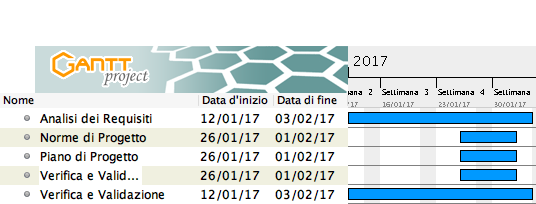
\includegraphics[scale=0.6]{Immagini/Gantt/ARD.png}
	\caption{Diagramma di Gantt, \ARD}
\end{figure}

\subsection{\PA}
Periodo: dal 06/02/2017 al 21/02/2017 \\

Inizia in seguito alla terminazione dell'\ARD\ ed il suo il termine prefissato coincide con una \termine{milestone} interna.
Il \termine{gruppo} si pone l'obbiettivo di eseguire la progettazione del sistema ad alto livello e di redigere il documento \ST.\\
In quest'ultimo documento i \ProgP\ dovranno descrivere, ad alto livello, le scelte progettuali ed il \termine{design-pattern} scelti per la realizzazione dell'architettura generale del \termine{prodotto}. Vengono inoltre incrementati i documenti \NdP, \PdP, \PdQ\ e \Gl.\\
In questa fase i ruoli maggiormente interessati sono: \Prog, \Pm, \Ver\ e \Am.

 \begin{figure}[H]
	\centering 
	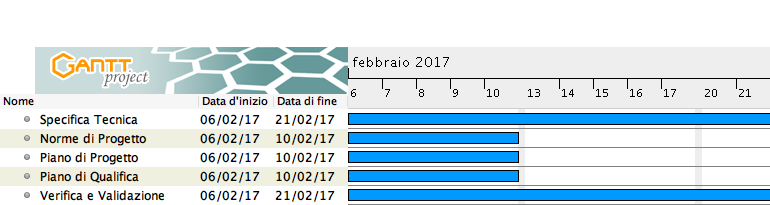
\includegraphics[scale=0.6]{Immagini/Gantt/PA.png}
	\caption{Diagramma di Gantt, \PA}
\end{figure}

\subsection{\PD}
Periodo: dal 22/02/2017 all'08/03/2017\\

Questa fase inizia in seguito all'approvazione della \PA\ e termina con una \termine{milestone} esterna che coincide con la consegna dei documenti per la \RP.\\
Il gruppo si impegna ad intraprendere e completare le seguenti attività:
\begin{itemize}
\item
Redigere il documento \DDP\ in cui i \ProgrP\ e i \ProgP\ devono descrivere il comportamento e le interazioni tra i vari componenti del sistema, basandosi sul documento di \ST;
\item
Incrementare i documenti \NdP, \PdP, \PdQ, \ST\ e \Gl.
\end{itemize}
In questa fase i ruoli maggiormente impegnati sono quelli di \Prog, \Pm, \Ver\ e \Am.

 \begin{figure}[H]
	\centering 
	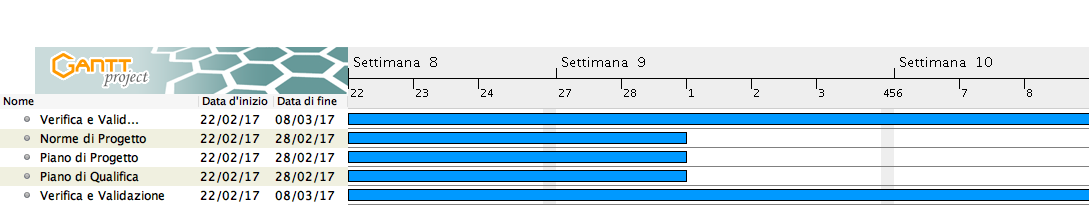
\includegraphics[scale=0.4]{Immagini/Gantt/PD.png}
	\caption{Diagramma di Gantt, \PD}
\end{figure}

\subsubsection{\COD}
Periodo: dal 14/03/2017 all'11/04/2017. \\

Il periodo di \COD\ inizia una volta concluso quello di \PD, e si conclude con la consegna del prodotto alla \RQ. L'obiettivo in questo periodo consiste nel consegnare un prodotto completo, e le attività che verranno eseguite in questa fase a tal fine sono le seguenti:
\begin{itemize}
	\item \COD: i \ProgrP\ dovranno sviluppare il codice del prodotto software attenendosi il più possibile a quanto scritto dai \ProgP\ nel documento \DDP. L'attività di \COD\ deve essere fatta seguendo, iterativamente, i seguenti passi fino all realizzazione del prodotto finito:
			\begin{itemize}
				\item \termine{Codifica} dell'incremento svolto dai \ProgP;
				\item \termine{Verifica} dell'incremento;
			\end{itemize}
	\item Stesura \MU: questo documento è destinato all'utilizzatore finale del prodotto che, tramite esso, deve essere in grado di capire le principali funzionalità del sistema e come utilizzarle;
	\item Incremento dei documenti \NdP, \PdP, \PdQ\ e \Gl;
	\item \termine{Verifica} dei documenti sopra citati.
\end{itemize}
In questa fase i ruoli maggiormente interessati sono quelli di \Am, \Pm, \Prog, \Progr\ e \Ver.

 \begin{figure}[H]
	\centering 
	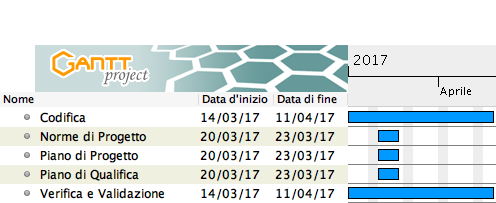
\includegraphics[scale=0.6]{Immagini/Gantt/COD.png}
	\caption{Diagramma di Gantt, \COD}
\end{figure}

\subsubsection{Verifica e Validazione}
Periodo: dal 16/12/2016 al 14/05/2017.\\

Questa fase, come si può osservare dalla data di inizio, è trasversale a tutti i periodi. Infatti, per garantire ad ogni incremento efficacia ed efficienza del prodotto, le operazioni di \termine{testing}, \termine{verifica} e \termine{validazione} vengono eseguite durante tutto il corso del progetto.\\

\paragraph{\VV}
Periodo: dal 12/04/2017 al 15/05/2017 \\

Al termine della \COD\ verranno effettuati ed intensificati tutti i test necessari per garantire che il prodotto soddisfi tutti i requisiti dell'\AdR.
Le attività prevedono di:
\begin{itemize}
	\item Effettuare dei test di sistema;
	\item Incrementare i documenti di: \MU, \NdP, \PdP, \PdQ\ e \Gl;
	\item Verificare tutti i documenti sopra citati.
\end{itemize}
In questa fase i ruoli maggiormente interessati sono quelli di \Ver, \Prog, \Am\ e \Pm.

 \begin{figure}[H]
	\centering 
	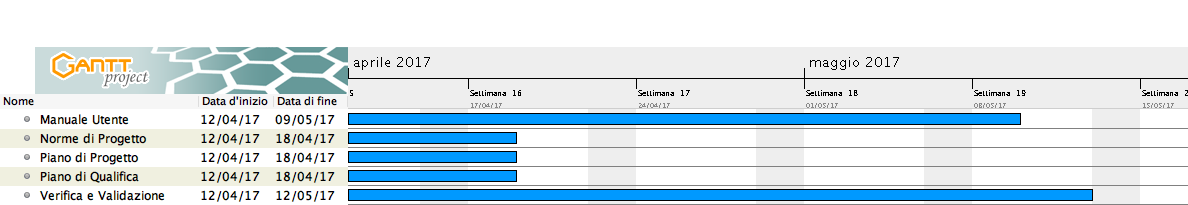
\includegraphics[scale=0.4]{Immagini/Gantt/VV.png}
	\caption{Diagramma di Gantt, \VV}
\end{figure}